\documentclass[10pt,a4paper]{article} 
\usepackage[czech]{babel}
\usepackage[utf8]{inputenc}
\usepackage[T1]{fontenc}
\usepackage{lmodern}
\usepackage{amssymb}
\usepackage{amsmath}
\usepackage[margin=2cm]{geometry}
\usepackage{pgfplots}
\usepackage{nicefrac}
\pgfplotsset{width=10cm,compat=1.9}
\usepackage{tikz}
\usetikzlibrary{patterns, arrows}
\usepackage{enumitem}
\usepackage{graphicx}
\usepackage{mathrsfs}
\usepackage{float}

\title{Domácí úkol číslo 1 nejlegendárnějšího týmečku A}
\author{Přibyl, Volák, Brada, Nawrath, Štancl}

\begin{document}
	\maketitle
	Náš tým se shodl na nejlepším softwaru jako na geogebře. 
	
	Začneme vytvořením obrázku reprezentující úlohu v geogebře. Je důležité použít \uv{Geogebra classic}, jiné tuto funkci nenabízejí: 
	
	\begin{figure}[H] 
		\centering
		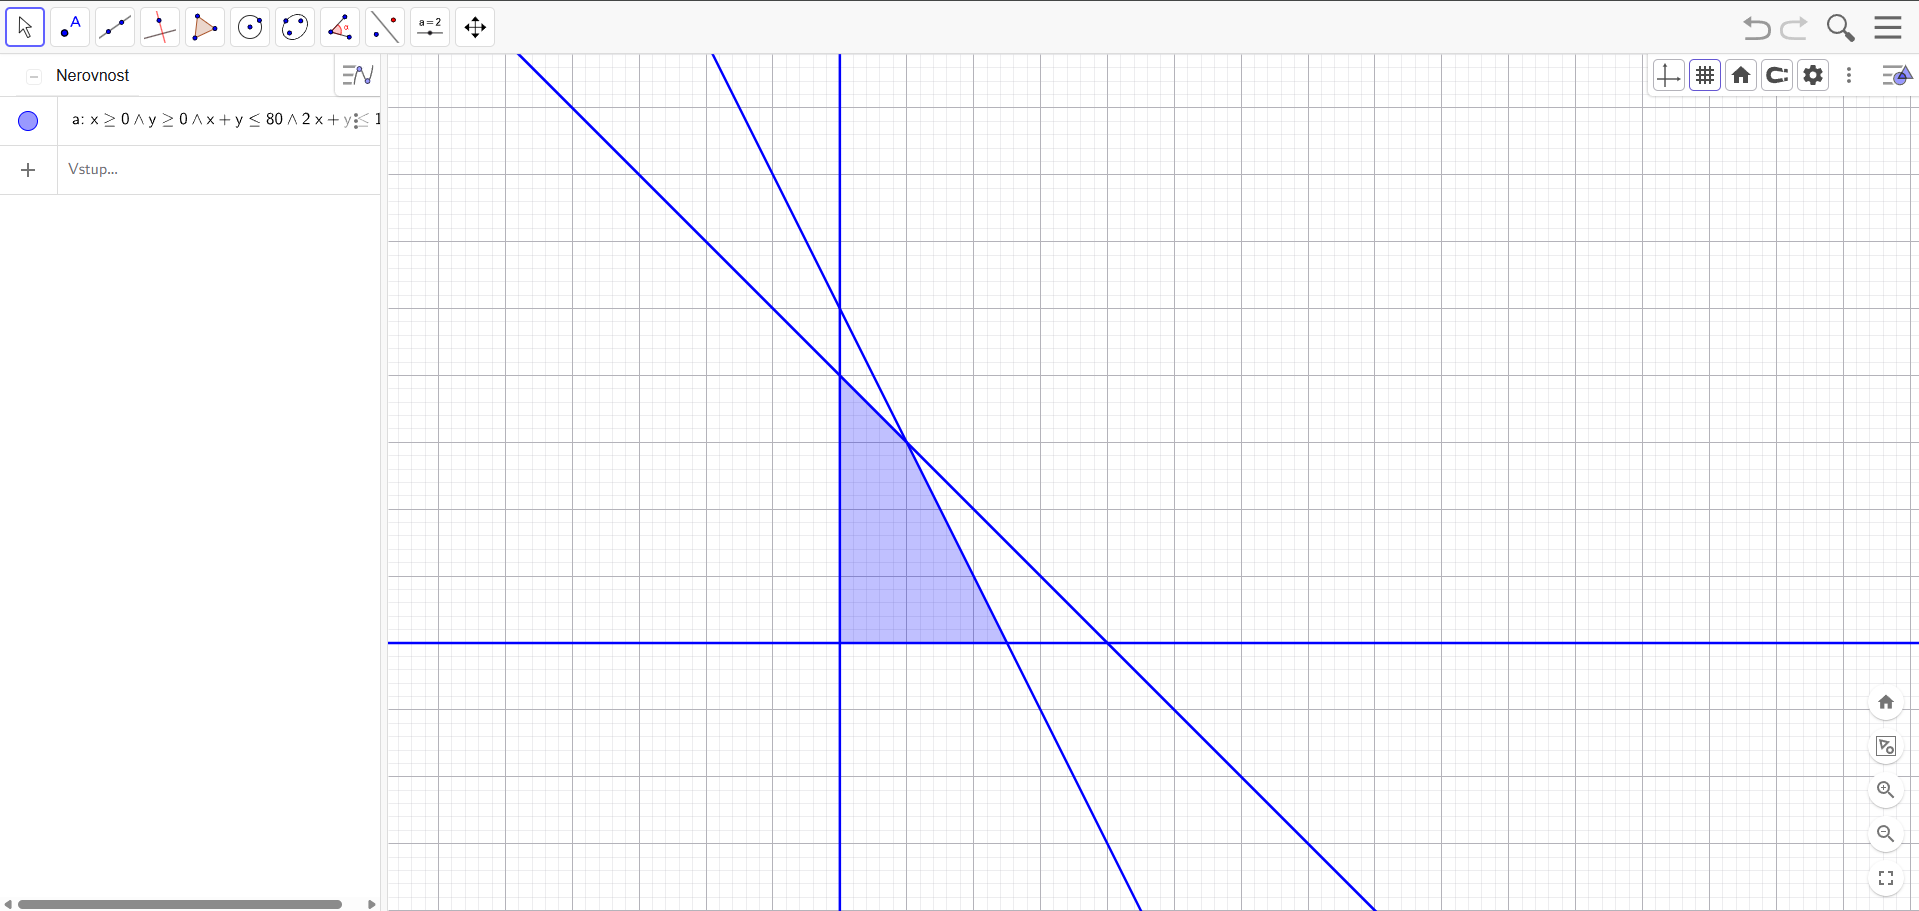
\includegraphics[width=0.7\linewidth]{screenshot003}
		\caption{Prostředí Geogebra Classic}
		\label{fig:screenshot003}
	\end{figure}
	
	Po vytvoření klikneme na možnost \uv{Stáhnout jako...} a podmožnost \uv{PGF/TikZ (.txt)}:
	
	\begin{figure}[H]
		\centering
		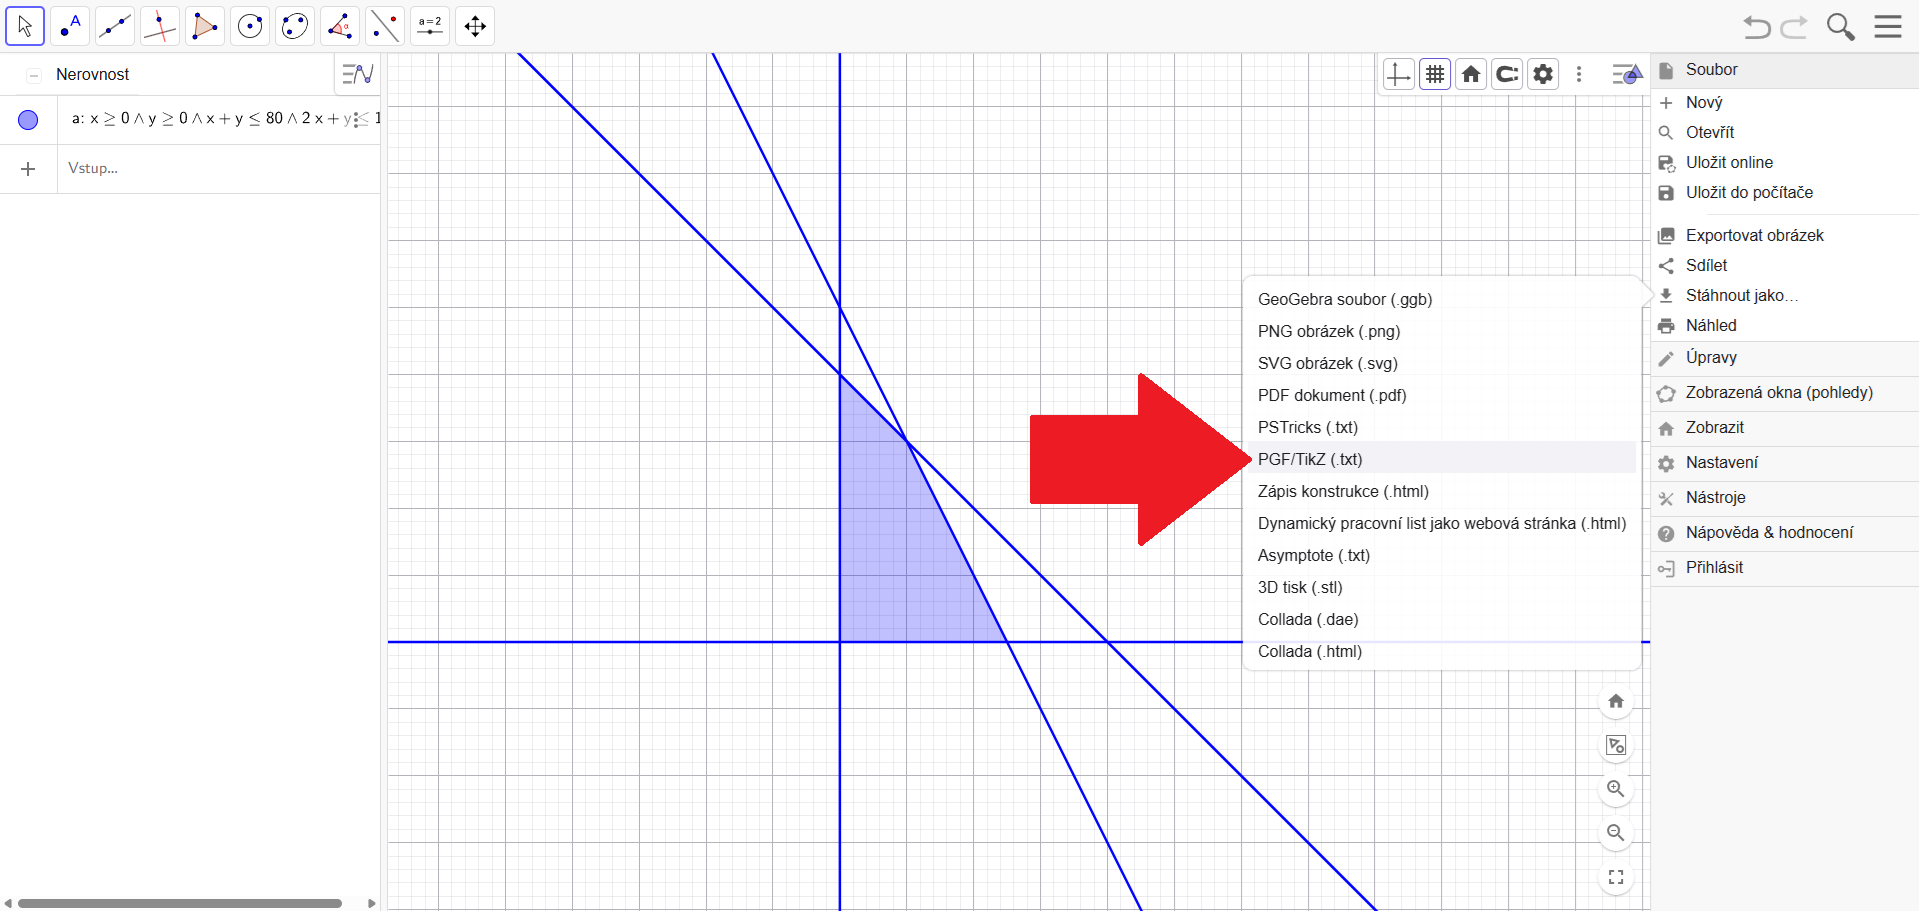
\includegraphics[width=0.7\linewidth]{screenshot004}
		\caption{Export do TikZ}
		\label{fig:screenshot004}
	\end{figure}
	
	Zvolíme název stahovaného souboru. Pozor, pokud se již soubor tohoto jména ve složce nachází, přidá se k názvu před tečku a označení formátu $(n)$, kde $n$ je pořadové číslo tohoto souboru: 
	
	\begin{figure}[H]
		\centering
		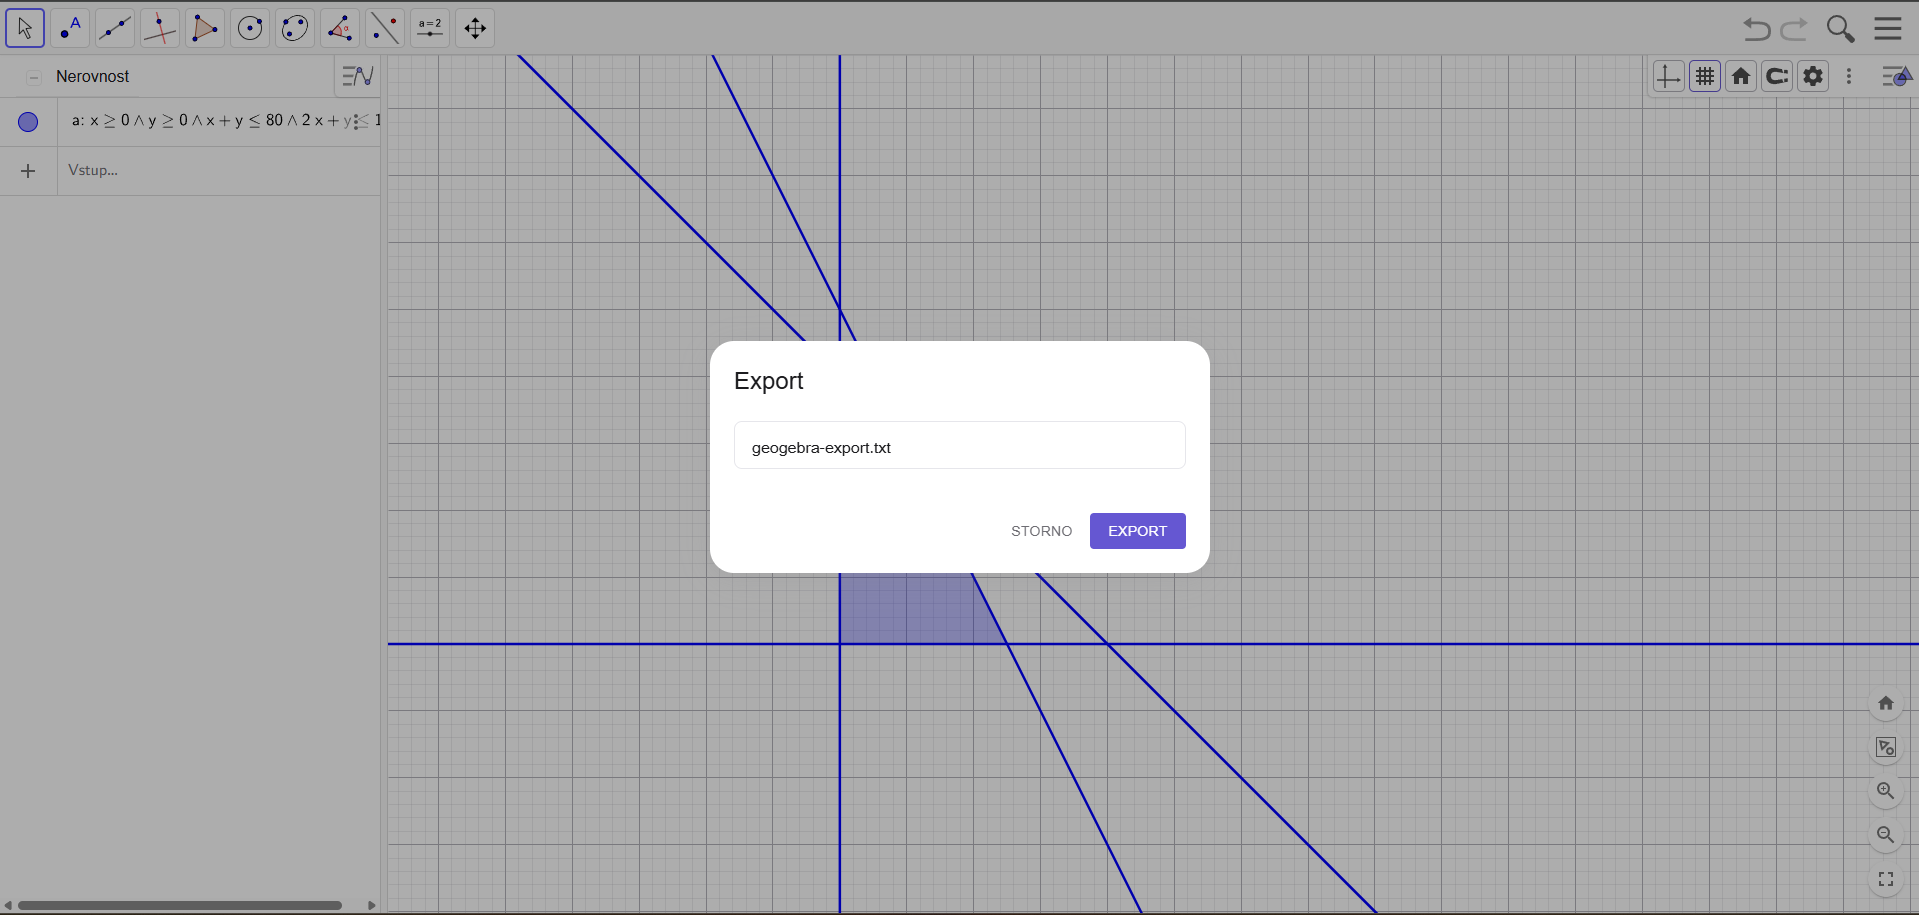
\includegraphics[width=0.7\linewidth]{screenshot005}
		\caption{Uložení souboru}
		\label{fig:screenshot005}
	\end{figure}
	
	Obsah souboru bude vypadat asi jako:
	
	\begin{figure}[H]
		\centering
		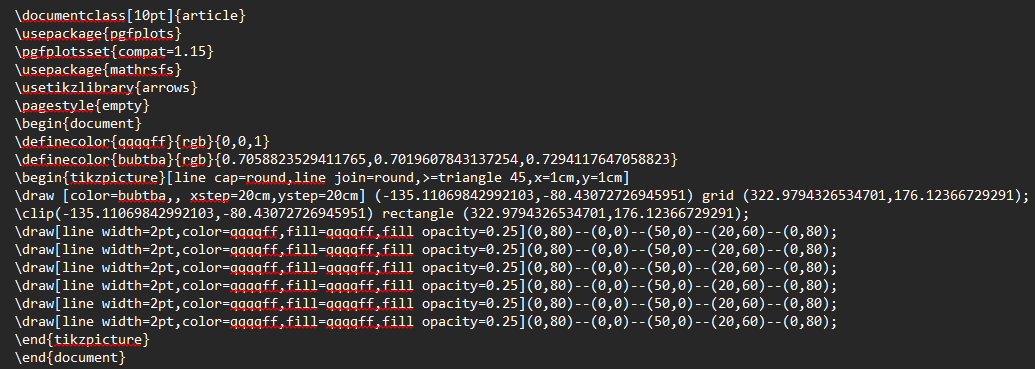
\includegraphics[width=0.7\linewidth]{screenshot006}
		\caption{Ukázka vygenerovaného kódu}
		\label{fig:screenshot006}
	\end{figure}
	
	Nyní jsou před vámi dvě možnosti: 
	
	\begin{enumerate}
		\item Jste masochisté a rádi hlídáte importované knihovny. Pak vám stačí modlit se a zkopírovat kód v sekci dokument. V našem případě vzniklo konkrétně toto (aby fungovalo, bylo nutno to začarovat kouzly dávných druidů):
		
		\begin{center} 
			\definecolor{qqqqff}{rgb}{0,0,1}
			\definecolor{bubtba}{rgb}{0.7058823529411765,0.7019607843137254,0.7294117647058823}
			\begin{tikzpicture}[line cap=round, line join=round, >=triangle 45, x=0.1cm, y=0.1cm]
				\clip (-10,-10) rectangle (60,90);
				\draw [color=bubtba, xstep=20, ystep=20] (-10,-10) grid (60,90);
				\draw[line width=2pt, color=qqqqff, fill=qqqqff, fill opacity=0.25] 
				(0,80) -- (0,0) -- (50,0) -- (20,60) -- cycle;
				\foreach \x in {20,40,60} \draw (\x,1) -- (\x,-1) node[below, scale=0.7] {\x};
				\foreach \y in {20,40,60,80} \draw (1,\y) -- (-1,\y) node[left, scale=0.7] {\y};
				\node[below left] at (0,0) {0};
			\end{tikzpicture}
		\end{center}
		
		\item Pokud ale máte náznaky lásky ke svému volnému času, jde to i za pomocí příkazu \texttt{\textbackslash input}. Nevýhodou je, že program je méně transparentní a hůře se tam něco mění, ale pokud člověk potřebuje rychle hodně obrázků, je to jednodušší. 
		
		\centering
		 \input{geogebra-export.txt}
	\end{enumerate}
\end{document}